%% This is file `sample-sigconf.tex',
%% generated with the docstrip utility.
%%
%% The original source files were:
%%
%% samples.dtx  (with options: `sigconf')
% TODO: Change to review before submitting
\documentclass[sigconf]{acmart}
%% \BibTeX command to typeset BibTeX logo in the docs
\AtBeginDocument{%
  \providecommand\BibTeX{{%
    \normalfont B\kern-0.5em{\scshape i\kern-0.25em b}\kern-0.8em\TeX}}}

%% Rights management information.  This information is sent to you
%% when you complete the rights form.  These commands have SAMPLE
%% values in them; it is your responsibility as an author to replace
%% the commands and values with those provided to you when you
%% complete the rights form.
\setcopyright{acmcopyright}
\copyrightyear{2018}
\acmYear{2018}
\acmDOI{XXXXXXX.XXXXXXX}

%% These commands are for a PROCEEDINGS abstract or paper.
\acmConference[ICSE 2024]{46th International Conference on Software Engineering}{April 2024}{Lisbon, Portugal}
%
%  Uncomment \acmBooktitle if th title of the proceedings is different
%  from ``Proceedings of ...''!
%
%\acmBooktitle{Woodstock '18: ACM Symposium on Neural Gaze Detection,
%  June 03--05, 2018, Woodstock, NY} 
\acmPrice{15.00}
\acmISBN{978-1-4503-XXXX-X/18/06}


%%
%% end of the preamble, start of the body of the document source.
\begin{document}

%%
%% The "title" command has an optional parameter,
%% allowing the author to define a "short title" to be used in page headers.
\title{The Name of the Title is Hope}

%%
%% The "author" command and its associated commands are used to define
%% the authors and their affiliations.
%% Of note is the shared affiliation of the first two authors, and the
%% "authornote" and "authornotemark" commands
%% used to denote shared contribution to the research.
\author{Ben Trovato}
\authornote{Both authors contributed equally to this research.}
\email{trovato@corporation.com}
\orcid{1234-5678-9012}
\author{G.K.M. Tobin}
\authornotemark[1]
\email{webmaster@marysville-ohio.com}
\affiliation{%
  \institution{Institute for Clarity in Documentation}
  \streetaddress{P.O. Box 1212}
  \city{Dublin}
  \state{Ohio}
  \country{USA}
  \postcode{43017-6221}
}

\author{Lars Th{\o}rv{\"a}ld}
\affiliation{%
  \institution{The Th{\o}rv{\"a}ld Group}
  \streetaddress{1 Th{\o}rv{\"a}ld Circle}
  \city{Hekla}
  \country{Iceland}}
\email{larst@affiliation.org}

\author{Valerie B\'eranger}
\affiliation{%
  \institution{Inria Paris-Rocquencourt}
  \city{Rocquencourt}
  \country{France}
}

\author{Aparna Patel}
\affiliation{%
 \institution{Rajiv Gandhi University}
 \streetaddress{Rono-Hills}
 \city{Doimukh}
 \state{Arunachal Pradesh}
 \country{India}}

\author{Huifen Chan}
\affiliation{%
  \institution{Tsinghua University}
  \streetaddress{30 Shuangqing Rd}
  \city{Haidian Qu}
  \state{Beijing Shi}
  \country{China}}

\author{Charles Palmer}
\affiliation{%
  \institution{Palmer Research Laboratories}
  \streetaddress{8600 Datapoint Drive}
  \city{San Antonio}
  \state{Texas}
  \country{USA}
  \postcode{78229}}
\email{cpalmer@prl.com}

\author{John Smith}
\affiliation{%
  \institution{The Th{\o}rv{\"a}ld Group}
  \streetaddress{1 Th{\o}rv{\"a}ld Circle}
  \city{Hekla}
  \country{Iceland}}
\email{jsmith@affiliation.org}

\author{Julius P. Kumquat}
\affiliation{%
  \institution{The Kumquat Consortium}
  \city{New York}
  \country{USA}}
\email{jpkumquat@consortium.net}

%%
%% By default, the full list of authors will be used in the page
%% headers. Often, this list is too long, and will overlap
%% other information printed in the page headers. This command allows
%% the author to define a more concise list
%% of authors' names for this purpose.
\renewcommand{\shortauthors}{Trovato and Tobin, et al.}

%%
%% The abstract is a short summary of the work to be presented in the
%% article.
\begin{abstract}
  TODO: Abstract
\end{abstract}

%%
%% The code below is generated by the tool at http://dl.acm.org/ccs.cfm.
%% Please copy and paste the code instead of the example below.
%%
\begin{CCSXML}
<ccs2012>
 <concept>
  <concept_id>00000000.0000000.0000000</concept_id>
  <concept_desc>Do Not Use This Code, Generate the Correct Terms for Your Paper</concept_desc>
  <concept_significance>500</concept_significance>
 </concept>
 <concept>
  <concept_id>00000000.00000000.00000000</concept_id>
  <concept_desc>Do Not Use This Code, Generate the Correct Terms for Your Paper</concept_desc>
  <concept_significance>300</concept_significance>
 </concept>
 <concept>
  <concept_id>00000000.00000000.00000000</concept_id>
  <concept_desc>Do Not Use This Code, Generate the Correct Terms for Your Paper</concept_desc>
  <concept_significance>100</concept_significance>
 </concept>
 <concept>
  <concept_id>00000000.00000000.00000000</concept_id>
  <concept_desc>Do Not Use This Code, Generate the Correct Terms for Your Paper</concept_desc>
  <concept_significance>100</concept_significance>
 </concept>
</ccs2012>
\end{CCSXML}

\ccsdesc[500]{Do Not Use This Code~Generate the Correct Terms for Your Paper}
\ccsdesc[300]{Do Not Use This Code~Generate the Correct Terms for Your Paper}
\ccsdesc{Do Not Use This Code~Generate the Correct Terms for Your Paper}
\ccsdesc[100]{Do Not Use This Code~Generate the Correct Terms for Your Paper}

%%
%% Keywords. The author(s) should pick words that accurately describe
%% the work being presented. Separate the keywords with commas.
\keywords{Debugging, Visual Debugging, Visual Debugger, IntelliJ IDEA Plugin, Software Maintenance, Software Visualization}

\received{9 November 2023}
% \received[revised]{12 March 2009}
% \received[accepted]{5 June 2009}

\maketitle

\section{Introduction}

\begin{figure}[ht]
  \centering
  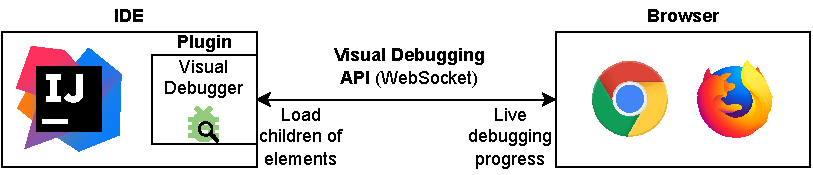
\includegraphics[width=\linewidth]{images/VD-architecture.pdf}
  \caption{Pic}
\end{figure}

\cite{krauterVisualDebuggerTool2022}

% \section{Acknowledgments}

\bibliographystyle{ACM-Reference-Format}
\bibliography{bib}
\end{document}
\endinput
%%
%% End of file `sample-sigconf.tex'.
